\documentclass[aspectratio=169,10pt]{beamer}
\usetheme{Madrid}
\usecolortheme{seahorse}
\usefonttheme{professionalfonts}

\setbeamertemplate{footline}[frame number]
\setbeamertemplate{navigation symbols}{}

\usepackage{amsmath,amssymb,amsthm}
\usepackage{graphicx}
\usepackage{listings}
\usepackage{xcolor}
\usepackage{bm}
\usepackage{booktabs}
\usepackage{tikz}
\usetikzlibrary{arrows.meta,positioning,calc}

\graphicspath{{figures/}}

\lstdefinestyle{mystyle}{
    basicstyle=\ttfamily\scriptsize,
    numbers=left,
    numberstyle=\tiny\color{gray},
    frame=single,
    backgroundcolor=\color{gray!7},
    commentstyle=\color{green!50!black}\itshape,
    keywordstyle=\color{blue!70!black}\bfseries,
    stringstyle=\color{orange!70!black},
    breaklines=true,
    showstringspaces=false,
    tabsize=2,
    language=Python
}
\lstset{style=mystyle}

\newcommand{\bE}{\mathbb{E}}
\newcommand{\bP}{\mathbb{P}}
\newcommand{\bQ}{\mathbb{Q}}
\newcommand{\bR}{\mathbb{R}}
\newcommand{\cP}{\mathcal{P}}
\newcommand{\cQ}{\mathcal{Q}}
\newcommand{\cE}{\mathfrak{E}}
\newcommand{\Conv}{\mathrm{Conv}}
\newcommand{\KL}{\mathrm{KL}}

\title[E-Values -- Ch.6]{Hypothesis Testing with E-Values}
\subtitle{Chapter 6: The Log-Optimal E-Value and Reverse Information Projection}
\author{Based on Ramdas \& Wang}
\date{}

\begin{document}

% =====================================================================
\begin{frame}
\titlepage
\end{frame}

% =====================================================================
\begin{frame}{Where we are}
\begin{itemize}
\item Chapter 5: \textbf{universal inference} builds a valid e-variable
$E^{\mathrm{UI}} = q(Z)/p_{\max}(Z)$ for a composite null $\cP$ against
a point alternative $\cQ$ -- easy to construct, but only
\emph{asymptotically} log-optimal.
\item Chapter 6's question: does a genuinely \textbf{finite-sample
log-optimal} e-variable exist for composite $\cP$? Answer: \textbf{yes},
it is unique, it is called the \textbf{numeraire}, and it always
dominates universal inference.
\item The price: the numeraire is characterized through a
\textbf{duality theory} -- the numeraire on one side is paired with a
special sub-probability distribution, the \textbf{reverse information
projection (RIPr)}, on the other.
\item Setting fixed for this chapter: composite null $\cP$, \textbf{point}
alternative $\bQ$ (mixtures/plug-ins for composite alternatives were
Chapter 3.7's business).
\end{itemize}
\end{frame}

% =====================================================================
\begin{frame}[allowframebreaks]{Notation you'll need}

\begin{block}{Numeraire (plain meaning)}
Among all valid e-variables for testing $\cP$, the \textbf{numeraire}
$E^*$ is the single ``best'' or \textbf{reference} e-variable: the one
that maximizes worst-case expected log-growth (e-power) under the true
data-generating law $\bQ$. Think of it as the ``gold-standard currency''
against which every other e-variable's performance is measured --
that is literally why it is called a numeraire (a reference unit of
value, as in economics).
\end{block}

\begin{block}{Reverse information projection (RIPr) -- plain meaning}
The RIPr $\bP^*$ is the distribution inside (the closure/bipolar of)
the null $\cP$ that is ``closest'' to $\bQ$ as measured by
Kullback--Leibler (KL) divergence. It is called \emph{reverse}
because ordinarily one projects a complicated object onto a simpler
model in the argument order $\KL(\text{model}, \text{truth})$; here
we project $\bQ$ onto $\cP$ in the order $\KL(\bQ, \bP)$, with $\bQ$
appearing \emph{first} -- ``reversed'' relative to the classical
information projection.
\end{block}

\framebreak

\begin{block}{Convex duality / strong duality -- with an analogy}
\textbf{Convex duality} pairs a minimization problem with a maximization
problem such that the max is always $\le$ the min (``weak duality'').
\textbf{Strong duality} says that under nice conditions (convexity,
compactness, etc.) the two values \emph{coincide exactly}.

\emph{1-D analogy:} imagine two hikers approaching the same mountain
pass from opposite sides of a valley. One hiker walks \emph{downhill}
from a high peak (minimizing altitude), the other walks \emph{uphill}
from the valley floor (maximizing altitude). Weak duality just says
the uphill hiker's altitude never exceeds the downhill hiker's. Strong
duality is the pleasant surprise that, at the pass, both hikers end up
at \emph{exactly the same point} -- min from one side equals max from
the other. In Chapter 6:
\[
\underbrace{\max_{E \in \cE} \bE^{\bQ}[\log E]}_{\text{best e-power, from the ``e-variable side''}}
\;=\;
\underbrace{\min_{\bP \in \Conv(\cP)} \KL(\bQ,\bP)}_{\text{closest null distribution, from the ``distribution side''}}.
\]
\end{block}

\framebreak

\begin{block}{Bayes factor -- recap}
For simple hypotheses $p$ vs.\ $q$, the Bayes factor is the likelihood
ratio $B = q(Z)/p(Z)$. For \emph{composite} hypotheses with priors
$\mu$ (over $\cQ$) and $\nu$ (over $\cP$),
\[
B_n = \frac{\int_{\cQ} \prod_{i=1}^n q(X_i)\,\mu(\mathrm{d}q)}
{\int_{\cP} \prod_{i=1}^n p(X_i)\,\nu(\mathrm{d}p)}.
\]
$B_n$ is an e-variable \emph{only if} nature itself drew the null from
the prior $\nu$ -- an assumption frequentists are unwilling to make in
general. Chapter 6 will show exactly when/how the numeraire coincides
with (or beats) $B_n$.
\end{block}

\begin{block}{The set of e-variables $\cE$}
Throughout, $\cE = \{E \ge 0 : \bE^{\bP}[E] \le 1 \text{ for all } \bP \in \cP\}$:
all nonnegative random variables whose expectation is $\le 1$ under
\emph{every} distribution consistent with the null.
\end{block}
\end{frame}

% =====================================================================
\begin{frame}{6.1 The numeraire e-variable: definition}

\textbf{Intuition first.} If we could see the truth $\bQ$, we would use
the likelihood ratio $\mathrm{d}\bQ/\mathrm{d}\bP$ as our e-variable when
the null is simple $\cP=\{\bP\}$ -- it is unbeatable (Neyman--Pearson).
When $\cP$ is composite, is there still a single ``best e-variable for
every purpose''? Definition 6.1 says: yes, if we require it to beat
every other e-variable \emph{in ratio, on average under $\bQ$}.

\begin{block}{Definition 6.1: numeraire e-variable}
A \emph{numeraire} $E^*$ is a $\bQ$-almost-surely strictly positive
e-variable such that
\[
\bE^{\bQ}\!\left[\frac{E}{E^*}\right] \le 1 \quad \text{for every e-variable } E \in \cE.
\]
Symbols: $\bQ$ is the (point) alternative; $E, E^*$ are e-variables
(nonnegative, $\bE^{\bP}[E]\le 1$ $\forall \bP \in \cP$); the ratio
condition says no other e-variable can, on $\bQ$-average, exceed $E^*$
by more than a wash.
\end{block}

Compare to Definition 3.1's ordinary optimality notions: this is a much
stronger, ``uniformly best in ratio'' requirement, not just best in
expectation of $E$ itself.
\end{frame}

% =====================================================================
\begin{frame}{Uniqueness of the numeraire}

\textbf{Step-by-step proof that numeraires are $\bQ$-a.s.\ unique.}
Suppose $E_1^*, E_2^*$ are both numeraires. Let $Y = E_2^*/E_1^*$.

\begin{enumerate}
\item Apply the numeraire property of $E_1^*$ with $E = E_2^*$:
$\bE^{\bQ}[Y] = \bE^{\bQ}[E_2^*/E_1^*] \le 1$, so $1/\bE^{\bQ}[Y] \ge 1$.
\item Jensen's inequality (convexity of $x \mapsto 1/x$):
$1/\bE^{\bQ}[Y] \le \bE^{\bQ}[1/Y]$.
\item Apply the numeraire property of $E_2^*$ with $E = E_1^*$:
$\bE^{\bQ}[1/Y] = \bE^{\bQ}[E_1^*/E_2^*] \le 1$.
\end{enumerate}
Chaining: $1 \le 1/\bE^{\bQ}[Y] \le \bE^{\bQ}[1/Y] \le 1$. All
inequalities are equalities, so Jensen's inequality holds with equality
$\Rightarrow$ $Y$ is $\bQ$-a.s.\ \emph{constant}, and since
$\bE^{\bQ}[Y]=1$ that constant is $1$. Hence $E_1^* = E_2^*$,
$\bQ$-almost surely. We may therefore speak of \textbf{``the''}
numeraire.

\begin{block}{Simple null special case}
If $\cP = \{\bP\}$ is simple and $\bQ \ll \bP$, the numeraire is just
the likelihood ratio $E^* = \mathrm{d}\bQ/\mathrm{d}\bP$ -- exactly the
Neyman--Pearson optimal e-variable.
\end{block}
\end{frame}

% =====================================================================
\begin{frame}{Log-optimality and existence}

\begin{block}{Proposition 6.3: numeraire $\Leftrightarrow$ log-optimal}
A $\bQ$-a.s.\ strictly positive e-variable $E^*$ is a numeraire if and
only if it is \emph{log-optimal}:
\[
\bE^{\bQ}\!\left[\log \frac{E}{E^*}\right] \le 0 \quad \text{for every e-variable } E \in \cE.
\]
\end{block}

\emph{Why:} numeraire $\Rightarrow$ log-optimal follows from Jensen
($\log$ is concave) applied to the defining ratio inequality. The
converse uses a clever one-parameter family $E(t) = (1-t)E^* + tE$
(itself an e-variable for $t\in(0,1)$ by convexity of $\cE$), a
first-order Taylor argument as $t \downarrow 0$, and Fatou's lemma.

\begin{block}{Theorem 6.4: existence}
A numeraire \emph{always exists}, with no assumptions on $\cP,\bQ$
whatsoever. It is $\bQ$-a.s.\ finite if and only if
$\bQ \ll \cP$ (meaning: $\bQ(A)>0 \Rightarrow \sup_{\bP\in\cP}\bP(A)>0$
for every event $A$) -- a genuinely weak requirement, much weaker than
demanding a common dominating measure.
\end{block}
\end{frame}

% =====================================================================
\begin{frame}[fragile]{Python: numeraire property on a toy finite $\cP$}

\begin{lstlisting}
import numpy as np
# P = {P1, P2} two Bernoulli laws (null); Q = Bernoulli(0.8) (alternative).
# Verify E^Q[E / E*] <= 1 for several candidate e-variables E.
theta = np.array([0.3, 0.5])      # P1, P2 natural parameters (null)
q_theta, z = 0.8, np.array([0, 1])
def bern_pmf(z, th): return th**z * (1 - th)**(1 - z)
# candidate numeraire = LR of Q to the *largest* null point (6.7.2)
p_star = bern_pmf(z, theta.max())
q_pmf = bern_pmf(z, q_theta)
E_star = q_pmf / p_star
def is_e_variable(E):
    return all(np.sum(bern_pmf(z, th) * E) <= 1 + 1e-9 for th in theta)
candidates = {"E* itself": E_star, "constant 1": np.array([1.0, 1.0]),
              "LR to theta=0.3": q_pmf / bern_pmf(z, 0.3)}
for name, E in candidates.items():
    ratio = np.sum(q_pmf * (E / E_star))
    print(f"{name:18s} e-var={is_e_variable(E)!s:5s}  E^Q[E/E*]={ratio:.4f}")
\end{lstlisting}
\end{frame}

% =====================================================================
\begin{frame}{6.2 Strong duality for finite $\cP$: setup}

\textbf{Intuition.} When $\cP=\{\bP_1,\dots,\bP_K\}$ is finite, the set
of ``achievable null distributions'' $\Conv(\cP)$ (all mixtures
$\sum_k \lambda_k \bP_k$) is a nice compact convex set (a simplex
image). This is exactly the setting where strong duality theorems from
convex optimization apply cleanly.

\begin{block}{Proposition 6.5: weak duality (always true)}
For any e-variable $E \in \cE$ and any $\bP \in \Conv(\cP)$,
\[
\bE^{\bQ}[\log E] \le \KL(\bQ,\bP), \qquad \text{hence} \qquad
\sup_{E \in \cE} \bE^{\bQ}[\log E] \;\le\; \inf_{\bP \in \Conv(\cP)} \KL(\bQ,\bP).
\]
\emph{Derivation:} from $\log y \le y-1$, a change of measure gives
$\bE^{\bQ}[\log(E \, \mathrm{d}\bP^a/\mathrm{d}\bQ)] \le \bE^{\bP}[E]-1 \le 0$
for any $\bP\in\Conv(\cP)$; rearranging gives the displayed inequality.
This is the ``uphill hiker never above the downhill hiker'' half of
our analogy.
\end{block}
\end{frame}

% =====================================================================
\begin{frame}{6.2 Strong duality for finite $\cP$: the theorem}

\begin{block}{Proposition 6.6: strong duality (finite $\cP$)}
Suppose $\cP = \{\bP_1,\dots,\bP_K\}$, $\bP_k \ll \bQ$ for all $k$, and
$\min_{\bP \in \Conv(\cP)}\KL(\bQ,\bP) < \infty$. Then
\[
\bE^{\bQ}[\log E^*] \;=\; \max_{E\in\cE} \bE^{\bQ}[\log E]
\;=\; \min_{\bP \in \Conv(\cP)} \KL(\bQ,\bP) \;=\; \KL(\bQ,\bP^*),
\]
where $E^*$ is the numeraire and $\bP^*$ (the RIPr) achieves the
minimum.
\end{block}

\textbf{Why the min is attained.} Rewrite $\min_{\bP\in\Conv(\cP)}\KL(\bQ,\bP)$
as $\min_{\lambda \in \Delta_K} \KL\!\big(\bQ, \sum_{k=1}^K \lambda_k \bP_k\big)$,
a strictly convex minimization over the \emph{compact} simplex
$\Delta_K$ -- so a unique minimizer $\lambda^*$ exists, and
$\bP^* = \sum_k \lambda_k^* \bP_k$.
\end{frame}

% =====================================================================
\begin{frame}{6.2 Proof of strong duality, step by step}

\textbf{Goal:} exhibit \emph{one} e-variable whose e-power equals
$\KL(\bQ,\bP^*)$ -- by weak duality that e-variable must then be the
numeraire, and equality is forced.

\begin{enumerate}
\item Optimality of $\bP^*$ over the convex set
$\{\sum_k \lambda_k \bP_k : \lambda \in \Delta_K\}$ means for any
$\bP \in \cP$ and any mixing weight $\alpha \in [0,1]$,
\[
\KL(\bQ,\bP^*) = \min_{\alpha \in [0,1]} \KL\big(\bQ,\; \alpha \bP^* + (1-\alpha)\bP\big),
\]
i.e.\ $\alpha=1$ (pure $\bP^*$) already minimizes over this line segment.
\item First-order (KKT) condition at the boundary optimum $\alpha=1$:
moving from $\alpha=1$ toward $\alpha=0$ must not decrease the
objective, i.e.\ the derivative at $\alpha=1$ is $\ge 0$:
\[
-\bE^{\bQ}\!\left[\frac{\mathrm{d}(\bP^*-\bP)}{\mathrm{d}\bP^*}\right] \le 0
\iff
\bE^{\bQ}\!\left[\frac{\mathrm{d}\bP}{\mathrm{d}\bP^*}\right] \le 1
\iff
\bE^{\bP}\!\left[\frac{\mathrm{d}\bQ}{\mathrm{d}\bP^*}\right] \le 1.
\]
\item The last inequality says exactly: $\mathrm{d}\bQ/\mathrm{d}\bP^*$
is an e-variable (its $\bP$-expectation is $\le 1$ for every $\bP\in\cP$)!
\item By definition of e-power, the e-power of this e-variable is
$\bE^{\bQ}[\log(\mathrm{d}\bQ/\mathrm{d}\bP^*)] = \KL(\bQ,\bP^*)$.
\end{enumerate}
\textbf{Conclusion:} the numeraire is $E^* = \mathrm{d}\bQ/\mathrm{d}\bP^*$,
and its e-power equals $\KL(\bQ,\bP^*)$ -- matching the weak-duality
upper bound exactly. This is the ``two hikers meet at the pass'' moment.
\end{frame}

% =====================================================================
\begin{frame}{6.3 Reverse information projection: definition}

\textbf{Why we need to go beyond Section 6.2:} finiteness of $\cP$ gave
us compactness of $\Conv(\cP)$, so the minimizing $\bP^*$ was
guaranteed to exist \emph{inside} $\Conv(\cP)$. For general
(uncountable, non-dominated) $\cP$, this compactness is lost:
\begin{itemize}
\item the infimum KL divergence may not be attained inside $\Conv(\cP)$ at all;
\item the true minimizer may be a \emph{sub-probability measure}
(total mass $<1$), living strictly outside $\Conv(\cP)$;
\item without a common dominating measure, likelihood ratios and KL
divergences need care.
\end{itemize}

\begin{block}{Definition 6.7: Reverse information projection (RIPr)}
Let $E^*$ be the numeraire for $\cP$ against $\bQ$. The RIPr of $\bQ$
onto $\cP$, denoted $\bP^*$, is defined \emph{via the numeraire itself}:
\[
\frac{\mathrm{d}\bP^*}{\mathrm{d}\bQ} = \frac{1}{E^*},
\]
understood to be $0$ on the event $\{E^* = \infty\}$.
\end{block}
$\bP^*$ is unique up to $\bQ$-nullsets, satisfies $\bP^* \ll \bQ$, and
$\bP^*(\Omega) \le 1$ (so it is generally only a \emph{sub}-probability
measure) because $\bE^{\bQ}[1/E^*] \le 1$.
\end{frame}

% =====================================================================
\begin{frame}[allowframebreaks]{6.3.1 The effective null is the bipolar of $\cP$}

\textbf{Intuition.} The \emph{polar} of $\cP$ is just its set of
e-variables ($\cP^\circ = \cE$). Taking the polar \emph{again} (the
\emph{bipolar}) gives back the largest family of distributions
\emph{indistinguishable from $\cP$ using e-variables} -- call it the
\textbf{effective null}.

\begin{block}{Polar and bipolar}
\[
\cP^\circ = \{E \in \mathcal{X}_+ : \bE^{\bP}[E] \le 1 \ \forall \bP \in \cP\} = \cE,
\qquad
\cP^{\circ\circ} = \{\bP \in \mathcal{M}_+ : \bE^{\bP}[E] \le 1 \ \forall E \in \cP^\circ\}.
\]
Always $\cP^{\circ\circ} \cap \mathcal{M}_1 \supseteq \Conv(\cP)$, with
equality when $\cP$ is finite, but the inclusion can be \emph{strict}
in general.
\end{block}

\begin{block}{Example 6.8 (strict inclusion)}
$\cP$ = all unit-variance Gaussians with mean $<0$. The standard
Gaussian $N(0,1)$ is \emph{not} in $\Conv(\cP)$ (it's a boundary/limit
point), but it \emph{is} in $\cP^{\circ\circ}\cap\mathcal{M}_1$, which
in fact contains all unit-variance Gaussians with mean $\ge 0$.
\end{block}

\begin{block}{Theorem 6.10}
A powered e-variable for $\cP$ against $\bQ$ exists if and only if
$\bQ \notin \cP^{\circ\circ}$: the bipolar really is the largest set of
distributions e-variables cannot distinguish from the null.
\end{block}
\end{frame}

% =====================================================================
\begin{frame}[allowframebreaks]{6.3 The RIPr picture and general strong duality}

\begin{figure}
\centering
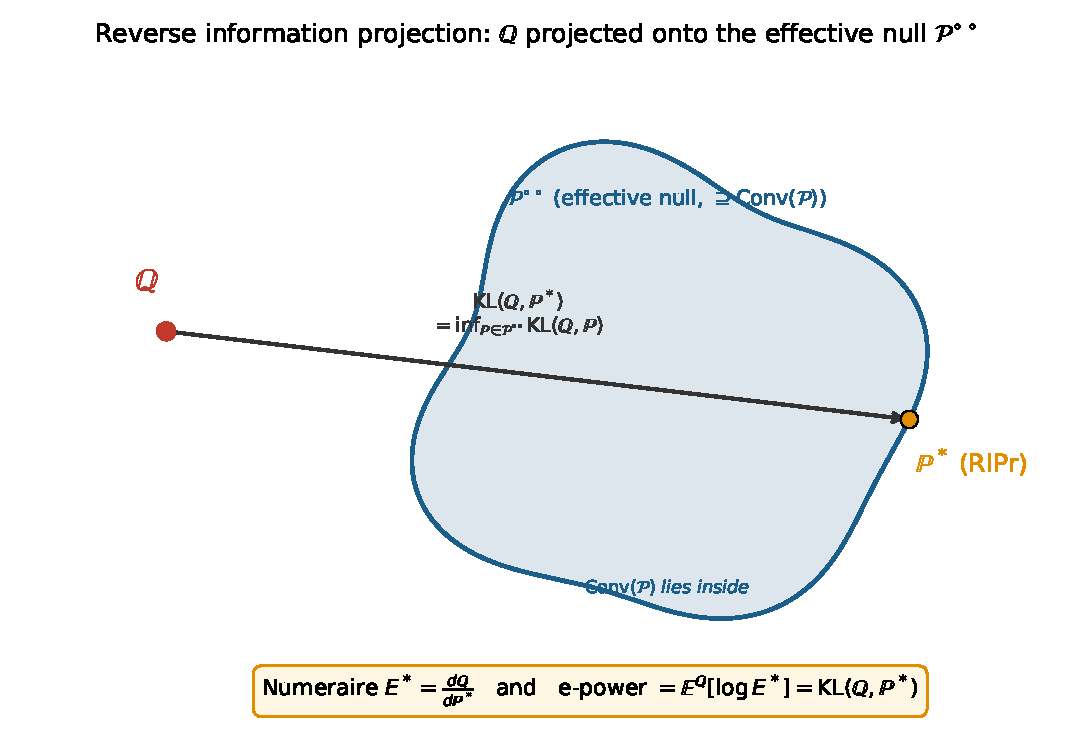
\includegraphics[width=0.62\textwidth]{fig_ripr_projection.pdf}
\end{figure}

\begin{block}{Proposition 6.11}
The RIPr always lies in the bipolar: $\bP^* \in \cP^{\circ\circ}$.
\end{block}

\begin{block}{Theorem 6.13: general strong duality (assuming $\bQ \ll \cP$)}
\[
\bE^{\bQ}[\log E^*] = \sup_{E \in \cE} \bE^{\bQ}[\log E]
= \inf_{\bP \in \cP^{\circ\circ}} \KL(\bQ,\bP) = \KL(\bQ,\bP^*),
\]
with no finiteness, dominance, or countability assumptions on $\cP$ --
the only change from Prop.\ 6.6 is that the infimum is now over the
\emph{bipolar} $\cP^{\circ\circ}$ instead of $\Conv(\cP)$, because that
is where the true minimizer may live.
\end{block}
\end{frame}

% =====================================================================
\begin{frame}[fragile]{Python: RIPr for a finite $\cP$ via convex optimization}

\begin{lstlisting}
import numpy as np
from scipy.optimize import minimize
# Finite P = {P1,P2,P3} on a small sample space, Q fixed. Solve
#   min_{lambda in simplex} KL(Q, sum_k lambda_k P_k)   ->  RIPr P*.
P = np.array([[0.6, 0.4], [0.3, 0.7], [0.5, 0.5]])  # rows P1,P2,P3
Q = np.array([0.2, 0.8])
def kl_objective(raw):
    w = np.exp(raw) / np.sum(np.exp(raw))         # softmax -> simplex
    return np.sum(Q * np.log(Q / (w @ P)))
res = minimize(kl_objective, x0=np.zeros(3), method="Nelder-Mead")
lam_star = np.exp(res.x) / np.sum(np.exp(res.x))
P_star = lam_star @ P
E_star = Q / P_star                                # numeraire = dQ/dP*
print("lambda* :", np.round(lam_star, 4))
print("RIPr P* :", np.round(P_star, 4))
print("E*      :", np.round(E_star, 4))
print("e-power = KL(Q,P*):", round(res.fun, 4))
for k in range(3):                                  # sanity: E^{P_k}[E*]<=1
    print(f"  E^P{k+1}[E*] = {np.sum(P[k]*E_star):.4f}")
\end{lstlisting}
\end{frame}

% =====================================================================
\begin{frame}{6.4 Numeraire is the only likelihood-ratio e-variable}

\textbf{Intuition.} The numeraire $E^* = \mathrm{d}\bQ/\mathrm{d}\bP^*$
is \emph{by construction} a likelihood ratio of $\bQ$ to some element
of the effective null. Theorem 6.15's surprise: it is the \textbf{only}
e-variable with this property. This gives a practical \textbf{recipe}:
guess a candidate likelihood ratio, verify it's a valid e-variable, and
you've automatically found the numeraire.

\begin{block}{Theorem 6.15 (verification theorem)}
Assume $\bQ \ll \cP$. Let $E^*$ be $\bQ$-a.s.\ strictly positive with
$\bP^*$ defined by $\mathrm{d}\bP^*/\mathrm{d}\bQ = 1/E^*$. Then:
$E^*$ is the numeraire $\iff$ $\bP^* \in \cP^{\circ\circ}$. Moreover
$\bE^{\bP^*}[E^*]=1$ and $\bP^*$ is \emph{maximal}: no other
$\bP \in \cP^{\circ\circ}$ equivalent to $\bQ$ dominates it setwise.
\end{block}

\begin{block}{Corollary 6.16 (practical recipe)}
If $\cP = \{\bP \in \mathcal{M}_1 : \bE^{\bP}[E]\le 1 \ \forall E \in \cE_0\}$
for a generating family $\cE_0$, and a candidate $E^*>0$ satisfies
$\bE^{\bQ}[1/E^*] = 1$ and $\bE^{\bQ}[E/E^*] \le 1$ for all $E \in \cE_0$,
then $E^*$ \emph{is} the numeraire.
\end{block}

\emph{Lemma 6.17 (shrinking):} if $\bP^*$ still belongs to the bipolar
of a \emph{smaller} null $\overline{\cP} \subseteq \cP$, the same $E^*$
remains the numeraire for $\overline{\cP}$ too -- dual to the lifting
lemma (6.2) for enlarging $\cP$.
\end{frame}

% =====================================================================
\begin{frame}{6.5 Numeraire dominates universal inference}

\textbf{Intuition.} Universal inference builds its e-variable from the
\emph{maximum likelihood over the whole null}, evaluated on the actual
data: $E^{\mathrm{UI}} = q(Z)/p_{\max}(Z)$ where
$p_{\max}(Z) = \sup_{p\in\cP} p(Z)$. Since the RIPr density $p^*$ is
itself just \emph{one} candidate inside (the bipolar of) $\cP$, we
always have $p^*(Z) \le p_{\max}(Z)$ -- so dividing by the
\emph{smaller} quantity $p^*$ gives a \emph{larger} e-variable.

\begin{block}{Domination}
\[
E^* = \frac{q(Z)}{p^*(Z)} \;\ge\; \frac{q(Z)}{p_{\max}(Z)} = E^{\mathrm{UI}}
\qquad \text{($\mathbb{L}$-almost surely)}.
\]
In nondegenerate composite-null cases the inequality is \emph{strict}
with positive probability -- so universal inference is
\textbf{inadmissible}: the numeraire is never worse, and is sometimes
strictly better, while requiring \emph{no} data splitting and no
reference measure at all (unlike UI, which needs densities).
\end{block}

\textbf{Coherence trade-off:} universal inference is \emph{logically
coherent} (enlarging the null can only weaken its e-variable); the
numeraire generally is \emph{not} coherent. More e-power, less
interpretability -- a genuine trade-off.
\end{frame}

% =====================================================================
\begin{frame}{Running example: coin fairness -- setting up the numbers}

\textbf{Story.} We test whether a coin is fair-or-biased-toward-tails,
$H_0: \theta \le 0.5$ (a \emph{composite}, ``robust'' null protecting
against any degree of tails-bias), versus the point alternative that
the coin has bias $\theta_1 = 0.7$ towards heads. We flip it $n=20$
times and observe $s=14$ heads.

\begin{block}{Bernoulli exponential family (Section 6.7.1/6.7.2 machinery)}
$p_\theta(z) = \theta^{z}(1-\theta)^{1-z}$ is a one-dimensional
exponential family with sufficient statistic $T(z)=z$ and natural
parameter monotone in $\theta$. For a one-sided null
$\Theta_0 = (-\infty,\theta_0]$ and point alternative $\theta_1>\theta_0$,
the RIPr is $p_{\theta_0}$ (the boundary point) and the numeraire is the
plain likelihood ratio to that boundary:
\[
E^* = \prod_{i=1}^n \frac{p_{\theta_1}(Z_i)}{p_{\theta_0}(Z_i)}
= \left(\frac{\theta_1}{\theta_0}\right)^{S}\left(\frac{1-\theta_1}{1-\theta_0}\right)^{n-S},
\qquad S = \textstyle\sum_i Z_i.
\]
\end{block}

With $\theta_0=0.5,\ \theta_1=0.7,\ n=20,\ S=14$:
\[
E^* = \left(\frac{0.7}{0.5}\right)^{14}\left(\frac{0.3}{0.5}\right)^{6}
= 1.4^{14}\times 0.6^{6} \approx 5.18.
\]
\end{frame}

% =====================================================================
\begin{frame}[allowframebreaks]{Running example: comparing to universal inference}

\textbf{Universal inference, done the way it is actually used in
practice} (Chapter 5): split the $n=20$ flips into a training half
(10 flips) and a test half (10 flips). Use the training half only to
estimate the boundary of the null (here: since the training data shows
more than 50\% heads, the restricted MLE sits exactly at the boundary
$\theta_0=0.5$); accumulate evidence only on the test half:
\[
E^{\mathrm{UI}} = \prod_{i \in \text{test}} \frac{p_{0.7}(Z_i)}{p_{0.5}(Z_i)}
= \left(\frac{0.7}{0.5}\right)^{s_2}\left(\frac{0.3}{0.5}\right)^{10-s_2}.
\]
With $s_2 = 7$ heads out of the 10 test flips (consistent with the
same overall 14/20):
\[
E^{\mathrm{UI}} = 1.4^{7}\times 0.6^{3} \approx 2.28.
\]

\begin{block}{Numbers side by side}
\begin{center}
\begin{tabular}{lcc}
\toprule
 & Numeraire $E^*$ (full sample) & Split-UI $E^{\mathrm{UI}}$ (test half only) \\
\midrule
Value & $\approx 5.18$ & $\approx 2.28$ \\
$\log$(value), nats & $1.646$ & $0.823$ \\
Data used & all 20 tosses & 10 tosses (10 ``spent'' on training) \\
\bottomrule
\end{tabular}
\end{center}
\end{block}
The numeraire is $E^*/E^{\mathrm{UI}} \approx 2.28\times$ larger here --
it never throws away data to estimate a training-set boundary,
because the RIPr theory handles the composite null for free.
\end{frame}

% =====================================================================
\begin{frame}[allowframebreaks]{Running example: e-power as a general curve}

In population terms, $\bE^{\bQ}[\log E^*] = n \cdot \KL(\theta_1\Vert\theta_0)$
(numeraire uses all $n$ flips) versus
$\bE^{\bQ}[\log E^{\mathrm{UI}}] = \tfrac{n}{2}\cdot \KL(\theta_1\Vert\theta_0)$
(split-UI only accrues evidence on the test half), where
\[
\KL(\theta_1\Vert\theta_0) = \theta_1 \log\frac{\theta_1}{\theta_0}
+ (1-\theta_1)\log\frac{1-\theta_1}{1-\theta_0}.
\]
For $\theta_1=0.7,\theta_0=0.5$: $\KL = 0.0823$ nats/flip, giving the
$1.646$ vs.\ $0.823$ nats above (a factor of exactly 2, the cost of
50/50 sample-splitting in this illustrative scheme).

\begin{figure}
\centering
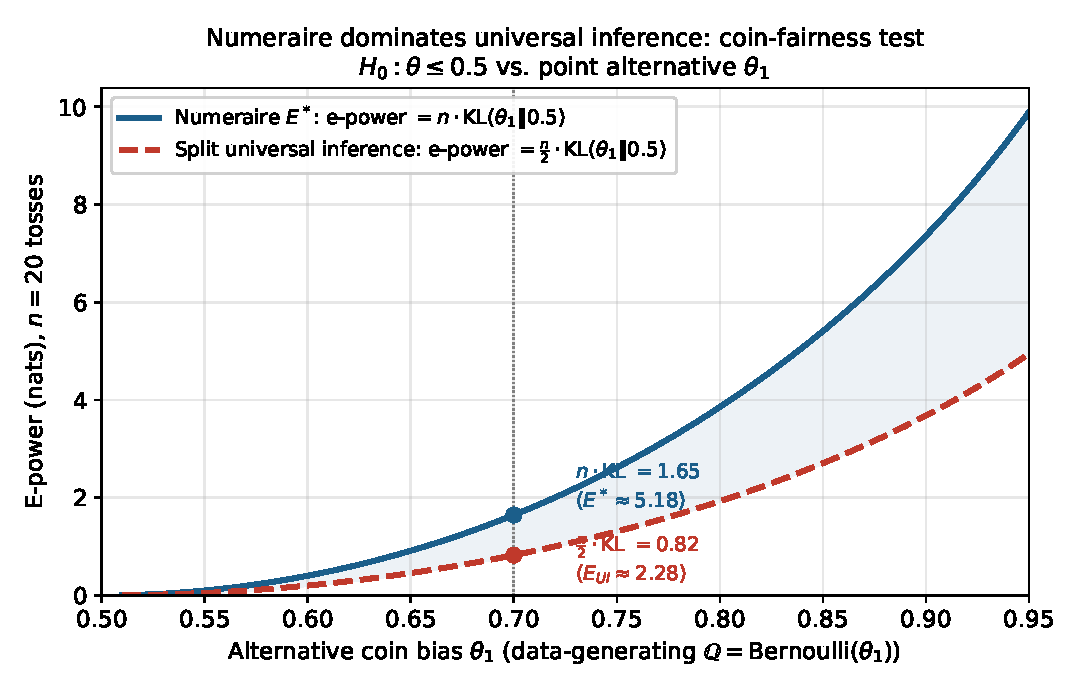
\includegraphics[width=0.72\textwidth]{fig_epower_domination.pdf}
\end{figure}
\end{frame}

% =====================================================================
\begin{frame}{6.6 E-values and Bayes factors}

\textbf{Intuition.} Four quantities compete to compare $\cQ$ vs.\ $\cP$
from data $X_1,\dots,X_n$: the Bayesian's Bayes factor, the
frequentist's generalized likelihood ratio, universal inference's
plug-in, and the numeraire. Only some of these are always valid
e-variables.

\begin{block}{Four competing statistics}
\[
B_n = \frac{\int_{\cQ}\prod_i q(X_i)\,\mu(\mathrm{d}q)}{\int_{\cP}\prod_i p(X_i)\,\nu(\mathrm{d}p)}
\ \ (\text{Bayes factor, priors } \mu,\nu),
\qquad
G_n = \frac{\sup_{q\in\cQ}\prod_i q(X_i)}{\sup_{p\in\cP}\prod_i p(X_i)}
\ \ (\text{generalized LR}),
\]
\[
U_n = \frac{\int_{\cQ}\prod_i q(X_i)\,\mu(\mathrm{d}q)}{\sup_{p\in\cP}\prod_i p(X_i)}
\ \ (\text{universal inference: mixture over } \cQ,\ \text{max over } \cP).
\]
\end{block}

\begin{itemize}
\item $B_n$ is an e-variable \emph{only if} nature really drew the null
from $\nu$ -- a strong, often unjustified assumption (internal but not
external consistency).
\item $G_n$ (Wilks' theorem) needs regularity conditions and only gives
an \emph{asymptotic} p-value.
\item $U_n$ is \emph{always} a valid e-variable, needing only densities
-- but is generally sub-optimal (Section 6.5).
\end{itemize}
\end{frame}

% =====================================================================
\begin{frame}[allowframebreaks]{6.6 The numeraire resolves all of this}

Define $\bQ^{\mathrm{eff}} = \int_{\cQ}\bQ^n\,\mu(\mathrm{d}\bQ)$ (a
mixture alternative) and let $\bP^*$ be its RIPr onto (the bipolar of)
$\{\bP^n : \bP\in\cP\}$. Then
\[
E_n = \frac{\mathrm{d}\bQ^{\mathrm{eff}}}{\mathrm{d}\bP^*}(X_1,\dots,X_n)
\]
is \emph{always} well defined -- even with no reference measures at all
for $\cP,\cQ$ -- is always a valid e-variable, and it \emph{dominates}
$U_n$.

\begin{block}{When do they coincide?}
\begin{itemize}
\item Both null and alternative simple: $B_n$, $U_n$, $E_n$ all coincide.
\item Only the null simple: Bayes factor, universal inference, and the
numeraire all coincide.
\item Neither simple: $B_n$ is only \emph{sometimes} an e-variable;
$E_n$ is only \emph{sometimes} representable as a Bayes factor (when
the RIPr lies inside $\Conv(\cP)$, i.e.\ is an actual mixture); $G_n$ is
generally neither an e-variable nor a Bayes factor.
\end{itemize}
\end{block}

The key insight: \emph{for every choice of alternative mixture, there
is a unique mixture over the null that reproduces the numeraire as a
literal Bayes factor} (Section 6.4) -- so the numeraire can be viewed
as ``the'' canonical, uniquely defensible Bayes factor, without needing
to justify a subjective prior over the null.
\end{frame}

% =====================================================================
\begin{frame}[fragile]{Python: $6.7$ examples -- computing all the numeraires}

\begin{lstlisting}
import numpy as np
# 6.7.1/6.7.2: exp. family, one-sided null theta<=theta0, point alt theta1
def numeraire_exp_family(theta0, theta1, S, n):
    return (theta1/theta0)**S * ((1-theta1)/(1-theta0))**(n-S)
print("Coin fairness E*:", round(numeraire_exp_family(0.5, 0.7, 14, 20), 4))

# 6.7.3: symmetry null;  E* = 2 q(z) / (q(z)+q(-z))
def numeraire_symmetry(qz, qmz):
    return 2*qz/(qz+qmz) if (qz+qmz) > 0 else 0.0

# 6.7.4: bounded-mean null {E[Z]<=mu}; E* = 1+lambda*(Z-mu), solve FOC
def solve_lambda_star(mu, grid=np.linspace(1e-6, 1/mu-1e-6, 20000)):
    foc = 1 - (1/grid)*np.log((1+grid*(1-mu))/(1-grid*mu))
    return grid[np.argmin(np.abs(foc))]

# 6.7.5: sub-Gaussian null; E* = exp(mu*Z - mu^2/2), lambda*=mu
def numeraire_subgaussian(z, mu):
    return np.exp(mu*z - mu**2/2)
print("Sub-Gaussian E* at z=1.5, mu=1:", round(numeraire_subgaussian(1.5, 1.0), 4))

# 6.7.6: LR-bounded null {dP/dP0<=gamma}; E* = (Z* v z0)/gamma
def numeraire_lr_bound(z_star, z0, gamma):
    return max(z_star, z0) / gamma
\end{lstlisting}
\end{frame}

% =====================================================================
\begin{frame}[allowframebreaks]{6.7.1--6.7.2 Exponential families \& monotone likelihood ratio}

\textbf{Intuition.} For exponential family nulls, restricting the
family to its ``worst-case boundary point'' turns out to give exactly
the RIPr -- a beautifully concrete instance of the abstract theory.

\begin{block}{Setup}
$p_\theta(z) = e^{\theta T(z) - A(\theta)}$ w.r.t.\ reference measure
$\mathbb{L}$, $A$ convex/differentiable, $T$ one-dimensional sufficient
statistic, natural parameter $\theta \in \Theta$. Null
$\cP = \{p_\theta : \theta \in \Theta_0\}$ with $\Theta_0$ closed,
largest element $\theta_0$; alternative $q = p_{\theta_1}$, $\theta_1>\theta_0$.
\end{block}

\textbf{Derivation that $p_{\theta_0}$ is the RIPr.} Using the moment
generating function of $T$,
\[
\bE^{\bQ}\!\left[\frac{p_\theta(Z)}{p_{\theta_0}(Z)}\right]
= e^{A(\theta_1+\theta-\theta_0) - A(\theta_1) - A(\theta) + A(\theta_0)}, \quad \theta \in \Theta_0.
\]
Any convex $f$ satisfies $f(a+b+c)-f(a+c) \ge f(b+c)-f(c)$ for $a,b\ge0$;
applying this to $f=A$ shows the exponent is $\le 0$, so the ratio is
$\le 1$ for all $\theta\in\Theta_0$ -- this is exactly condition (iv)
of Theorem 6.14, confirming $p_{\theta_0}$ is the RIPr. Hence
\[
E^* = \frac{p_{\theta_1}(Z)}{p_{\theta_0}(Z)} = e^{(\theta_1-\theta_0)T(Z) - A(\theta_1)+A(\theta_0)}.
\]
This is exactly our coin-fairness formula, and generalizes it: any
one-sided exponential family null makes the numeraire a simple
likelihood ratio to the boundary.
\end{frame}

% =====================================================================
\begin{frame}{6.7.3 Testing symmetry}

\textbf{Intuition.} Null: $Z \stackrel{d}{=} -Z$ (a symmetric, entirely
non-parametric, non-dominated family). A natural guess for the RIPr is
the symmetrization of $\bQ$, but because the symmetrized measure need
not equal $\bQ$ exactly on the support, we must take its
\emph{absolutely continuous part}.

\begin{block}{RIPr and numeraire for symmetry testing}
With $q$ the Lebesgue density of $\bQ$,
\[
p^*(z) = \tfrac12\big(q(z)+q(-z)\big)\,\mathbb{1}_{\{q(z)>0\}},
\qquad
E^* = \frac{\mathrm{d}\bQ}{\mathrm{d}\bP^*} = \frac{2\,q(Z)}{q(Z)+q(-Z)}\,\mathbb{1}_{\{q(Z)>0\}}.
\]
\end{block}

\textbf{Why this is the numeraire (sketch).} One shows the full set of
e-variables here is $\cE = \{E \le 1+\phi(Z): \phi \text{ odd}\}$
(any $E$ of this form has $\bE^{\bP}[E] \le 1+\bE^{\bP}[\phi(Z)]=1$
by symmetry). Writing $E^* = 1+\phi^*(Z)$ with
$\phi^*(z) = \frac{q(z)-q(-z)}{q(z)+q(-z)}$ (odd), a direct calculation
shows $\bE^{\bQ}[E/E^*] \le 1$ for every $E=1+\phi(Z)\in\cE$, confirming
the numeraire property.
\end{frame}

% =====================================================================
\begin{frame}[allowframebreaks]{6.7.4 Testing bounded means}

\textbf{Intuition.} Null: $Z \in [0,1]$ with mean $\le \mu$ -- a fully
nonparametric, non-dominated family (contains all point masses on
$[0,\mu]$!). Two obvious e-variables are $Z/\mu$ and the constant $1$;
any convex combination $1+\lambda(Z-\mu)$, $\lambda \in [0,1/\mu]$, is
also one. We search this family for the log-optimal choice.

\begin{block}{First-order condition (6.7)}
Maximizing $f(\lambda) = \bE^{\bQ}[\log(1+\lambda(Z-\mu))]$ (concave in
$\lambda$) over $\lambda \in [0,1/\mu]$ gives interior maximizer
$\lambda^*$ solving
\[
\bE^{\bQ}\!\left[\frac{Z-\mu}{1+\lambda^*(Z-\mu)}\right] = 0.
\]
For $\bQ = \mathrm{Uniform}[0,1]$ this reduces (via direct integration)
to the transcendental equation
\[
\frac{1+\lambda^*(1-\mu)}{1-\lambda^*\mu} = e^{\lambda^*},
\]
solved numerically. The resulting numeraire is
$E^* = 1+\lambda^*(Z-\mu)$, verified via Corollary 6.16 by checking
$\lambda=0$ and $\lambda=1/\mu$ satisfy the required inequality.
\end{block}
This shows the RIPr / numeraire machinery working even when \emph{no}
common exponential-family structure is available -- only a moment
constraint.
\end{frame}

% =====================================================================
\begin{frame}{6.7.5 \& 6.7.6 Sub-Gaussian means and likelihood-ratio bounds}

\begin{block}{6.7.5: Sub-Gaussian means}
Null: $Z$ is 1-sub-Gaussian with nonpositive mean,
$\cP = \{\bP : \bE^{\bP}[e^{\lambda Z - \lambda^2/2}] \le 1\ \forall \lambda\ge0\}$
(again non-dominated). Alternative $\bQ = N(\mu,1)$, $\mu>0$. Maximizing
$\bE^{\bQ}[\lambda Z-\lambda^2/2] = \lambda\mu-\lambda^2/2$ over
$\lambda\ge0$ gives $\lambda^*=\mu$, so
\[
E^* = e^{\mu Z - \mu^2/2}, \qquad \text{RIPr } \bP^* = N(0,1).
\]
\end{block}

\begin{block}{6.7.6: Testing likelihood-ratio bounds}
Null: $\cP=\{\bP: \mathrm{d}\bP/\mathrm{d}\bP_0 \le \gamma\}$ for fixed
$\bP_0,\gamma\ge1$. With $Z^*=\mathrm{d}\bQ/\mathrm{d}\bP_0$ and $z_0\ge0$
the largest constant with $\int_0^{1/\gamma}(q_t(Z^*)\vee z_0)\,\mathrm{d}t=1$
($q_t$ = left quantile function), the numeraire is
\[
E^* = \frac{Z^* \vee z_0}{\gamma}, \qquad
\frac{\mathrm{d}\bP^*}{\mathrm{d}\bP_0} = \gamma \wedge \frac{\gamma Z^*}{z_0}.
\]
The special case $\gamma=1$ recovers Theorem 3.20's log-optimal
e-variable for a simple null, with $z_0$ the largest constant that is
$\le Z^*$ a.s.\ (typically $z_0=0$).
\end{block}
\end{frame}

% =====================================================================
\begin{frame}{6.7.7 Testing exchangeability}

\textbf{Intuition.} Null: the data vector $Z=(Z_1,\dots,Z_n)$ is
\emph{exchangeable} (invariant in distribution under all permutations)
-- an infinite, non-parametric null with no common dominating measure
in general. This connects to permutation/rank tests.

\begin{block}{Numeraire via permutation averaging}
Let $\pi$ be uniform on the symmetric group $\mathcal{S}_n$, and $q$ the
density of the (non-exchangeable) alternative $\bQ$. Then
\[
E = \frac{q(Z)}{q(Z_\pi)} = \frac{q(Z)}{\frac{1}{n!}\sum_{\sigma\in\mathcal{S}_n} q(Z_\sigma)}
\]
is an e-variable for the exchangeability null. Because the distribution
with density $q(Z_\pi)$ (the permutation-symmetrized density) is itself
exchangeable -- hence lies in $\cP$ -- and $\mathrm{d}\bQ/\mathrm{d}\bP^*$
is the unique e-variable representable as a bipolar likelihood ratio
(Theorem 6.15), $E$ \emph{is} the numeraire, and $q(Z_\pi)$ is the RIPr.
\end{block}

This is a clean illustration of the ``guess-and-verify'' recipe from
Section 6.4: symmetrizing the alternative's density over all
permutations is the natural operation, and duality confirms it is
optimal, not just valid.
\end{frame}

% =====================================================================
\begin{frame}{Chapter 6 summary}
\begin{itemize}
\item The \textbf{numeraire} $E^*$ is the unique, finite-sample
log-optimal e-variable for composite $\cP$ against point $\bQ$; it
always exists.
\item It is dual to the \textbf{reverse information projection}
$\bP^*$: $E^* = \mathrm{d}\bQ/\mathrm{d}\bP^*$, and
$\bE^{\bQ}[\log E^*] = \KL(\bQ,\bP^*)$ -- \textbf{strong duality}
between maximizing e-power and minimizing KL divergence to the
\emph{effective null} $\cP^{\circ\circ}$ (the bipolar of $\cP$).
\item The numeraire is the \emph{only} e-variable expressible as a
likelihood ratio to an equivalent element of $\cP^{\circ\circ}$ --
enabling a practical guess-and-verify recipe (Corollary 6.16).
\item It always \textbf{dominates universal inference}
($E^* \ge E^{\mathrm{UI}}$), at the cost of losing logical coherence.
\item It unifies/subsumes Bayes factors, universal inference, and
(asymptotically) the generalized likelihood ratio, coinciding with
each under progressively simpler hypotheses.
\item Worked out explicitly for: exponential families, monotone
likelihood ratio families, symmetry, bounded means, sub-Gaussian
means, likelihood-ratio-bounded nulls, and exchangeability.
\end{itemize}
\end{frame}

\end{document}
